\documentclass[
    12pt,
    a4paper,
    oneside
]{article}

% -------------------------------------------------
% PACOTES
% -------------------------------------------------

\usepackage[brazil]{babel}
\usepackage[utf8]{inputenc}
\usepackage[T1]{fontenc}

\usepackage{times}
\usepackage{indentfirst}
\usepackage{graphicx}
\usepackage{float}
\usepackage{xcolor}
\usepackage{amsmath}
\usepackage{setspace}
\usepackage{geometry}
\usepackage{titlesec}
\usepackage{caption}

% -------------------------------------------------
% CONFIGURAÇÕES ABNT
% -------------------------------------------------

\geometry{
    a4paper,
    left=3cm,
    right=2cm,
    top=3cm,
    bottom=2cm
}

\setlength{\parindent}{1.25cm}
\setlength{\parskip}{0cm}

\onehalfspacing

% -------------------------------------------------
% INÍCIO DO DOCUMENTO
% -------------------------------------------------

\begin{document}

% -------------------------------------------------
% CAPA
% -------------------------------------------------

\begin{titlepage}

    \begin{minipage}[c]{0.3\textwidth}
        \raggedright
        \raisebox{0pt}[\height][0pt]{%
            
\includegraphics[width=4cm]{imagens/Logo_UnB.png}%
        }
    \end{minipage}
    \hfill
    \begin{minipage}[c]{0.7\textwidth}
        \centering
        \textbf{\LARGE Universidade de Brasília}\\[0.25cm]
        \textbf{\large Departamento de Ciência da Computação}\\[0.1cm]
    \end{minipage}

    \begin{center}
        \vspace{4cm}

        {\Large \textbf{Teleinformática e Redes 2}}

        \vspace{1cm}

        {\large Tarefa Camada de Transporte}

        \vfill

        \textbf{Membros}

        \vspace{0.5cm}

        Daniel Lincoln Lopes de Souza -- 202042829\\
        Isabela Soares Furlan -- 231013636\\
        Luiz Fernando Candido Soaris -- 190092025

        \vfill

        Brasília -- DF\\
        \today

    \end{center}

\end{titlepage}

% -------------------------------------------------
% SUMÁRIO
% -------------------------------------------------

\tableofcontents
\newpage

% -------------------------------------------------
% INTRODUÇÃO
% -------------------------------------------------

\section{Introdução}

Este relatório apresenta a análise de uma conexão TCP utilizando o Wireshark, com foco em mecanismos da camada de transporte. A partir da captura de tráfego e das ferramentas de análise disponíveis, foram investigados aspectos relacionados ao estabelecimento da conexão, transferência de dados, controle de congestionamento, retransmissões e desempenho da comunicação.

Os resultados obtidos permitiram observar o comportamento do protocolo TCP em uma sessão real e relacionar as evidências experimentais aos conceitos estudados na disciplina.

\section{Questões objetivas}

% Escreva aqui

\subsection{Questão 1}
O estabelecimento da conexão TCP foi identificado por meio do three-way handshake, composto pelos pacotes SYN, SYN-ACK e ACK observados no início do fluxo TCP analisado.

\subsubsection*{(a) RTT entre o SYN e o SYN-ACK}

O valor do RTT foi obtido diretamente do campo \textit{Time since previous frame in this TCP stream} presente no pacote SYN-ACK: \(0.220056629,\mathrm{s}\). Portanto, o tempo de ida e volta observado durante o estabelecimento da conexão foi de, aproximadamente: \(\mathrm{RTT}\approx220.06,\mathrm{ms}\)

\subsubsection*{(b) MSS negociado}

A análise das opções TCP do pacote SYN-ACK mostrou que o MSS (\textit{Maximum Segment Size}) negociado foi: \(\mathrm{MSS}=1416,\mathrm{bytes}\). Esse valor representa a quantidade máxima de dados úteis que podem ser transportados em um segmento TCP sem considerar os cabeçalhos dos protocolos inferiores.

\subsubsection*{(c) Janela inicial de recepção (rwnd)}

No pacote SYN-ACK, o servidor anunciou uma janela de recepção calculada (\textit{Calculated Window Size}) igual a: \(\mathrm{rwnd}=62636,\mathrm{bytes}\). Esse valor corresponde à quantidade de dados que o receptor estava apto a receber sem necessidade de confirmação adicional.

\subsubsection*{Evidência Experimental}

A Figura \ref{fig:handshake} apresenta os três pacotes do three-way handshake identificados na captura, bem como os campos relevantes expandidos no painel inferior do Wireshark.

\begin{figure}[H]
\centering
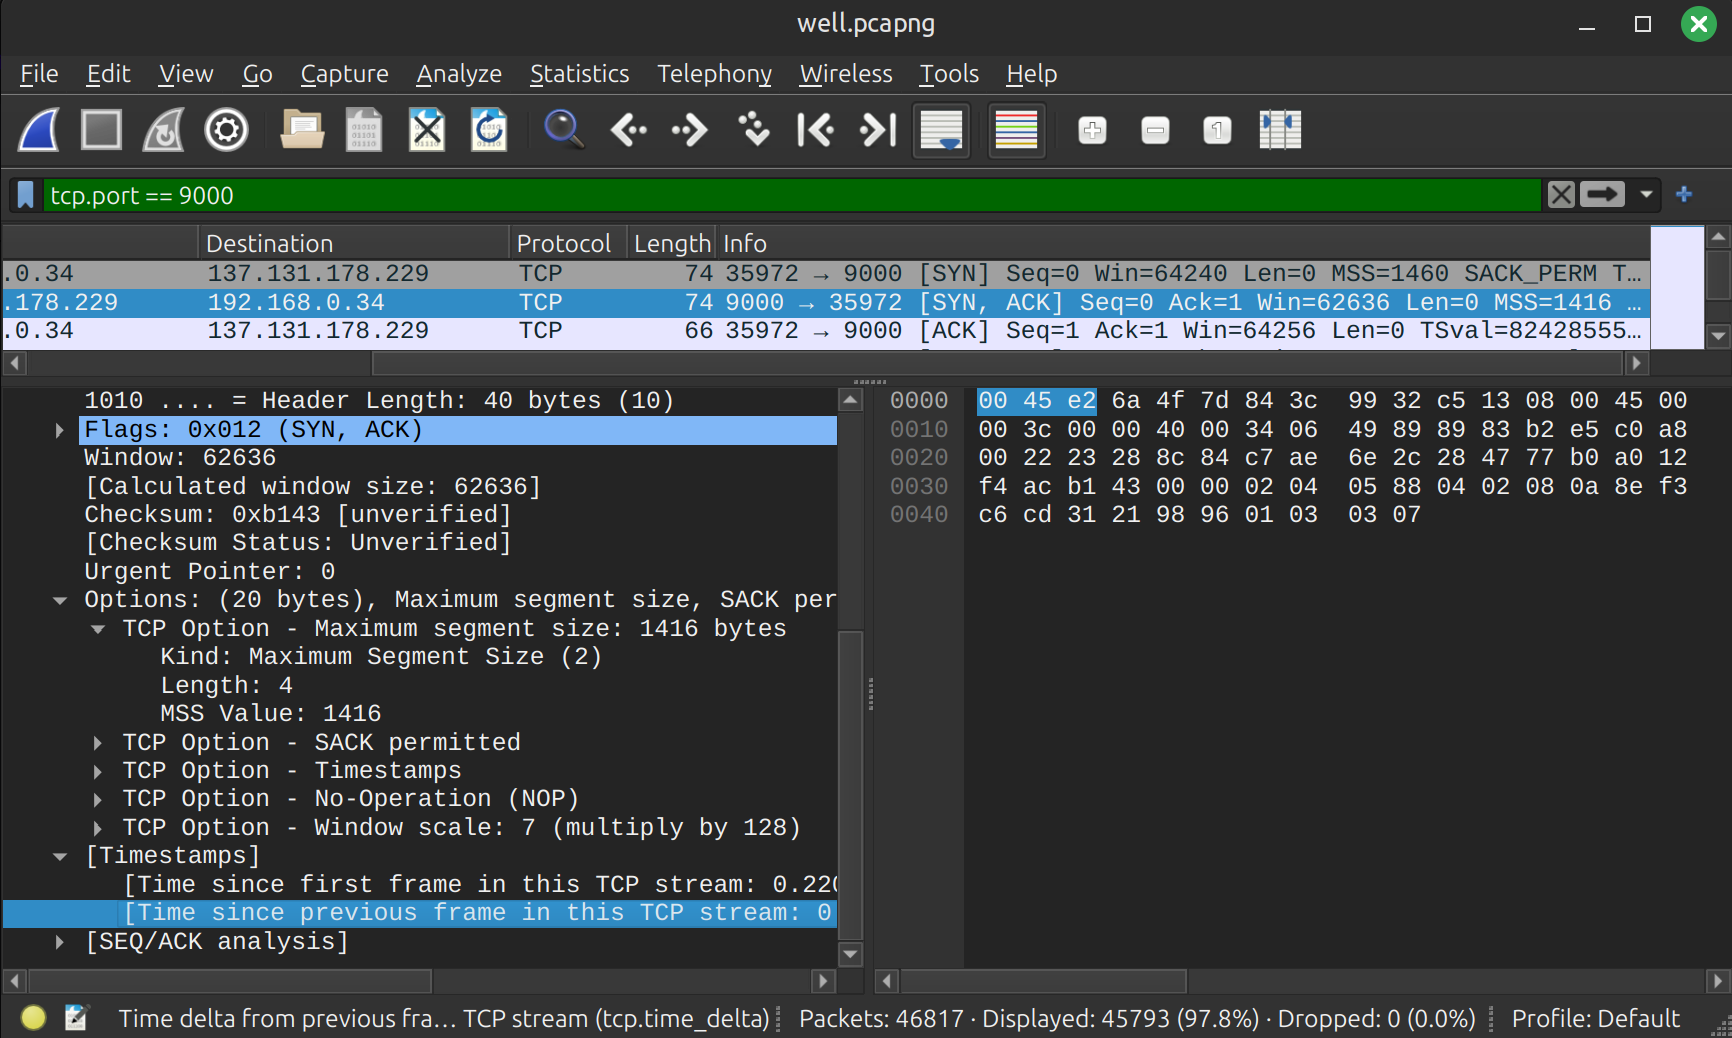
\includegraphics[width=0.8\textwidth]{figuras/q1-handshake.png}
\caption{Three-way handshake (SYN, SYN-ACK e ACK) com os campos TCP expandidos.}
\label{fig:handshake}
\end{figure}

\subsection{Questão 2}

% Escreva aqui

\subsection{Questão 3}

% Escreva aqui

\subsection{Questão 4}

% Escreva aqui

\subsection{Questão 5}
\subsubsection*{(a) Throughput médio reportado pelo cliente}

Ao final da execução do cliente foi apresentado o seguinte resumo:

\begin{verbatim}
Duração         : 60.0s
Total recebido  : 193.00 MB
Throughput médio: 3.22 MB/s
\end{verbatim}

O valor reportado foi: $3.22,\text{MB/s}$. Apesar de o programa utilizar o termo \textit{Throughput médio}, o valor medido pelo cliente está mais próximo de um \textit{goodput}, pois a aplicação contabiliza apenas os dados efetivamente recebidos pela aplicação de usuário. Dessa forma, cabeçalhos TCP, IP, Ethernet e eventuais retransmissões não fazem parte da quantidade de dados considerada pelo cliente.

\subsubsection*{(b) Vazão observada no Wireshark}

A ferramenta \textit{Statistics $\rightarrow$ Conversations (TCP)} apresentou os seguintes resultados para o fluxo analisado: Pacotes totais: 45793; Bytes totais: 267 MB; Pacotes A $\rightarrow$ B: 16394; Bytes A $\rightarrow$ B: 1 MB; Pacotes B $\rightarrow$ A: 29399; Bytes B $\rightarrow$ A: 266 MB; Taxa A $\rightarrow$ B: 143 kbps; Taxa B $\rightarrow$ A: 35 Mbps.

A taxa relevante para a transferência principal é a direção servidor $\rightarrow$ cliente (B $\rightarrow$ A), cujo valor médio foi aproximadamente: $35,\text{Mbps}$. A ferramenta \textit{Conversations} contabiliza os bytes observados na captura e, portanto, inclui o overhead dos protocolos observados durante a transmissão. Já o \textit{IO Graph} exibe a evolução temporal da taxa de transmissão ao longo da sessão, permitindo visualizar oscilações e períodos de maior ou menor utilização da rede.

\subsubsection*{(c) Comparação entre os valores}

Convertendo o valor informado pelo cliente para megabits por segundo: $3.22,\text{MB/s}\times8=25.76,\text{Mbps}$. Assim, $\text{Goodput}\approx25.76,\text{Mbps}$. Enquanto isso, o Wireshark indicou aproximadamente $\text{Throughput}\approx35,\text{Mbps}$. Os valores não são iguais. O valor obtido no Wireshark é maior porque considera não apenas os dados úteis entregues à aplicação, mas também os cabeçalhos dos protocolos e outros bytes transmitidos pela conexão TCP. Portanto, $\text{Throughput}>\text{Goodput}$, o que está de acordo com o comportamento esperado para uma transferência TCP real.

\subsubsection*{(d) Cálculo do overhead esperado}

Conforme indicado no enunciado, considera-se um payload de 1390 bytes por segmento, além de 20 bytes de cabeçalho TCP e 20 bytes de cabeçalho IP. O overhead total por segmento é, portanto, de 40 bytes.

Aplicando a fórmula fornecida:

$$\text{Overhead}(\%)=\frac{\text{Cabeçalhos}}{\text{Payload}+\text{Cabeçalhos}}\times100$$

$$\text{Overhead}(\%)=\frac{40}{1390+40}\times100$$

$$\text{Overhead}(\%)=\frac{40}{1430}\times100$$

$$\text{Overhead}(\%)\approx2.80\%$$

Portanto, espera-se que aproximadamente 2,8\% da capacidade transmitida seja consumida apenas pelos cabeçalhos TCP e IP. Entretanto, a diferença observada entre o throughput medido no Wireshark ($35,\text{Mbps}$) e o goodput medido pela aplicação ($25.76,\text{Mbps}$) foi significativamente maior que 2,8\%. Isso indica que, além dos cabeçalhos TCP/IP considerados no cálculo simplificado, outros fatores contribuíram para a diferença observada, como ACKs, controle de congestionamento, pausas introduzidas pelo servidor durante o experimento e possíveis retransmissões. Dessa forma, os resultados obtidos são compatíveis com o comportamento esperado de uma conexão TCP real, mas não podem ser explicados apenas pelos 40 bytes de cabeçalhos considerados no cálculo teórico.

\subsection*{Evidências Experimentais}

\begin{figure}[H]
\centering
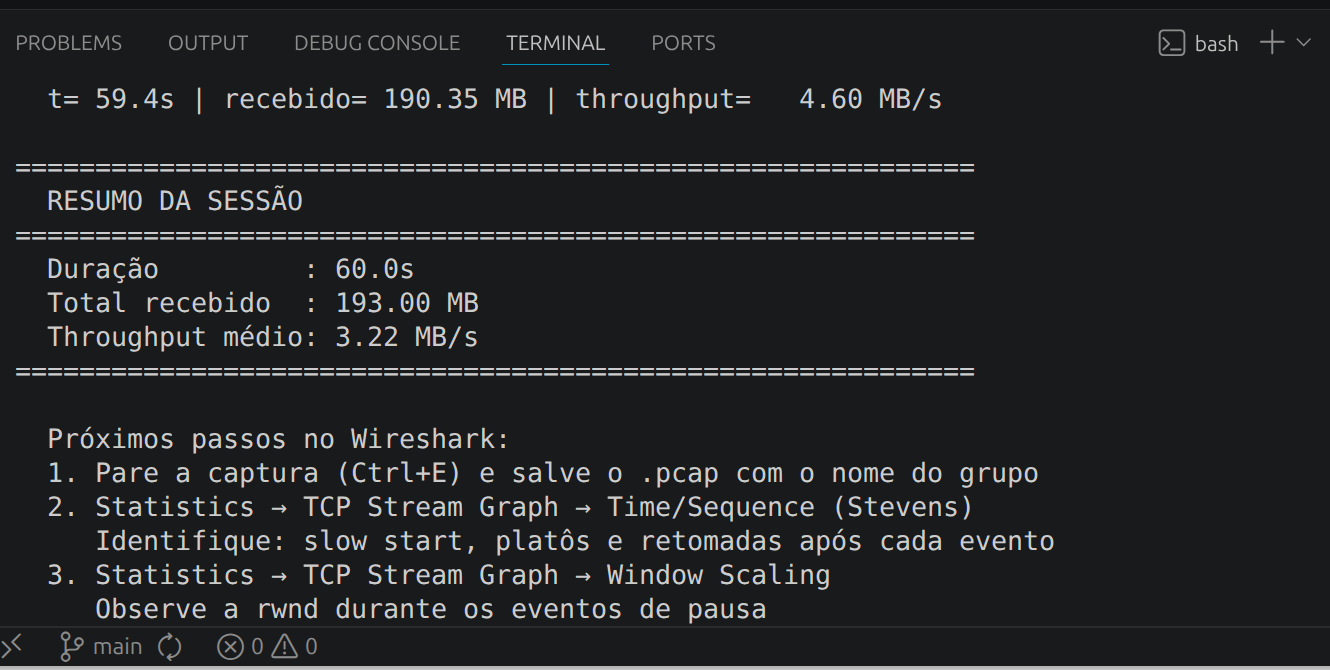
\includegraphics[width=0.85\textwidth]{figuras/q5-terminal.png}
\caption{Resumo da sessão exibido pelo cliente.}
\label{fig:q5terminal}
\end{figure}

\begin{figure}[H]
\centering
\includegraphics[width=0.85\textwidth]{figuras/q5-conversations.png}
\caption{Statistics $\rightarrow$ Conversations (TCP).}
\label{fig:q5conversations}
\end{figure}

\begin{figure}[H]
\centering
\includegraphics[width=0.85\textwidth]{figuras/q5-iograph.png}
\caption{Statistics $\rightarrow$ IO Graph com filtro tcp.stream eq 0.}
\label{fig:q5iograph}
\end{figure}

\section{Conclusão}

A captura analisada permitiu investigar diferentes mecanismos do protocolo TCP por meio de evidências obtidas no Wireshark e na aplicação cliente. Foram examinados aspectos relacionados ao estabelecimento da conexão, ao fluxo de dados, ao controle de congestionamento, às retransmissões e à vazão observada durante a transferência.

De modo geral, os resultados obtidos mostraram como conceitos teóricos da camada de transporte se manifestam em uma comunicação TCP real, evidenciando a utilidade de ferramentas de análise de tráfego para o estudo e diagnóstico de protocolos de rede.

\begin{thebibliography}{9}

\bibitem{tanenbaum}
TANENBAUM, Andrew S.;
WETHERALL, David J.
\textit{Redes de Computadores}.
5. ed.
São Paulo: Pearson, 2011.

\end{thebibliography}

\end{document}
